\documentclass {scrartcl}
\usepackage[a4paper, left=2.5cm, right=2.5cm, top=2.5cm, bottom=3cm]{geometry}
\usepackage[ngerman]{babel} % wegen deutschen Umlauten
\usepackage[utf8]{inputenc}
\usepackage{color}
\usepackage{listings}
\usepackage{fancyhdr}
\usepackage{graphicx}		% Einbinden von Bildern
\usepackage{ulem}				% Einbinden von Bildern
\usepackage{multicol} 	% Spalten
\usepackage{tipa} 			% Sonderzeichen wie | (pipe)
\usepackage{textcomp} 	% spitze klammern
\usepackage{rotating}
\usepackage{hyperref}   % hyperlinks
\usepackage{pdfpages}
\usepackage{subcaption}
\usepackage{float}
\usepackage{tikz}

%%%%%%%%%%%%%%%%%%%%%%%%%%%%%%%%%
% Adapt every excercise
%%%%%%%%%%%%%%%%%%%%%%%%%%%%%%%%%
\newcommand{\VersionNr}{2.0}
\newcommand{\Subject}{DC Motor Control}
\newcommand{\Name}{Lukas Rappel}
\newcommand{\Number}{S1510567014}


% Kopf-/Fußzeile
\pagestyle{fancy} %eigener Seitenstil

\fancyhf{} %alle Kopf- und Fußzeilenfelder bereinigen
\fancyhead[L]{Version \VersionNr} %Kopfzeile links
\fancyhead[C]{FH Hagenberg \\ \Subject} %zentrierte Kopfzeile
\fancyhead[R]{\Name\\ \Number} %Kopfzeile rechts
\renewcommand{\headrulewidth}{0.4pt} %obere Trennlinie
\fancyfoot[C] {-{\thepage}-} %Seitennummer
\renewcommand{\footrulewidth}{0.4pt} %untere Trennlinie
% C++ Source code
\definecolor{dkgreen}{rgb}{0,0.6,0}
\definecolor{gray}{rgb}{0.5,0.5,0.5}
\definecolor{mauve}{rgb}{0.58,0,0.82}
\setlength{\headheight}{26pt}
%%%%%%%%%%%%%%%%%%%%%%%% listings settings %%%%%%%%%%%%%%%%%%%%%%%%%%%%%%%
\lstset{ %
language=C++,                % choose the language of the code
basicstyle=\footnotesize\ttfamily,       % the size of the fonts that are used for the code
numbers=left,                   % where to put the line-numbers
numberstyle=\footnotesize,      % the size of the fonts that are used for the line-numbers
stepnumber=1,                   % the step between two line-numbers. If it is 1 each line will be numbered
numbersep=5pt,                  % how far the line-numbers are from the code
backgroundcolor=\color{white},  % choose the background color. You must add \usepackage{color}
showspaces=false,               % show spaces adding particular underscores
showstringspaces=false,         % underline spaces within strings
showtabs=false,                 % show tabs within strings adding particular underscores
frame=single,           				% adds a frame around the code
tabsize=4,          						% sets default tabsize to 2 spaces
captionpos=b,           				% sets the caption-position to bottom
breaklines=true,        				% sets automatic line breaking
breakatwhitespace=false,    		% sets if automatic breaks should only happen at whitespace
keywordstyle=\color{blue},      % keyword style
commentstyle=\color{dkgreen},   % comment style
stringstyle=\color{mauve}       % string literal style
%escapeinside={\%*}{*)}         % if you want to add a comment within your code
}
%%%%%%%%%%%%%%%%%%%%%%%% hyperlinks settings %%%%%%%%%%%%%%%%%%%%%%%%%%%%%%%
\hypersetup{colorlinks,
pdfstartview = FitH,
bookmarksopen = true,
bookmarksnumbered = true,
linkcolor = black,
plainpages = false,
hypertexnames = false,
citecolor = black
}

\lstset{
literate={ö}{{\"o}}1
{ä}{{\"a}}1
{ü}{{\"u}}1
{ß}{{\ss}}1
{é}{{\'e}}1,
inputencoding=ansinew,
extendedchars=true
}

%%%%%%%%%%%%%%% tikz
\usetikzlibrary{arrows}



\title {\Subject \\ \VersionNr}
\author {\Name (\Number)}
\date {\today}

\begin {document}
\tikzstyle{block} = [draw, fill=blue!20, rectangle, 
    minimum height=3em, minimum width=6em]
\tikzstyle{sum} = [draw, fill=blue!20, circle, node distance=1cm]
\tikzstyle{input} = [coordinate]
\tikzstyle{output} = [coordinate]
\tikzstyle{pinstyle} = [pin edge={to-,thin,black}]

\maketitle
\tableofcontents
\newpage
%%%%%%%%%%%%%%%%%%%%%%%%%%%%%%%%%%%%%%%%%%%%%%%%%%
\section{Overview}
A brief overview of contained IP-core is given in figure \ref{fig:block_IP}.
\begin{figure}[h]
	\centering
		\includegraphics{./Blockdiagram.PNG}
	\caption{block diagram of motor control IP Core}
	\label{fig:block_IP}
\end{figure}

\subsection{Design units}
The IP core is divided in several sub units. 
Design units can be found under \href {https://svn01.fh-hagenberg.at/projekte/SocGhostCar/trunk/04_software/fpga}{svn repository}

\begin{center}
  \begin{tabular}{ | l | l |}
	  \hline
		\textbf{Unit} & \textbf{Files} \\
		\hline
		top level (QSYS) & \url{/Motor_control/Motor_Control.vhd} \\
		Testbench & \url{/Motor_control/tbMotor_Control.vhd} \\
		\hline
		Round Sensor & \url{/Motor_control/RoundSensor/RoundSensor-e.vhd} \\
		Round Sensor & \url{/Motor_control/RoundSensor/RoundSensor-Rtl-a.vhd} \\
		Testbench & \url{/Motor_control/RoundSensor/tbRoundSensor.vhd} \\
		\hline
		Wheel Encoder & \url{/Motor_control/WheelEncoderTimer/WheelEncoderTimer-e.vhd} \\
		Wheel Encoder & \url{/Motor_control/WheelEncoderTimer/WheelEncoderTimer-Rtl-a.vhd} \\
		Testbench & \url{/Motor_control/WheelEncoderTimer/tbWheelEncoderTimer.vhd} \\
		\hline
		PWMGen, StrobeGen, .. & \url{/src} \\
		\hline
  \end{tabular} 
\end{center}

\subsection{External parts}
smart power fet, optical reflex wheel sensor, optical reflex round sensor


\section{QSYS Integration}
\begin{figure}[h]
	\centering
		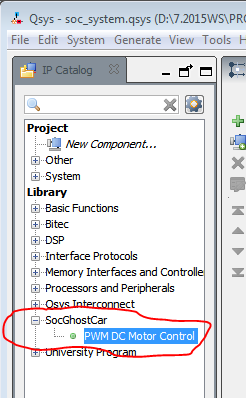
\includegraphics{./SocGhostCar_IP.png}
	\caption{Library SocGhostCar}
	\label{fig:SocGhostCar_IP}
\end{figure}

\subsection{QSYS Interface and Parameters}
Memory mapped slave interface is used.

\begin{figure}[h]
	\centering
		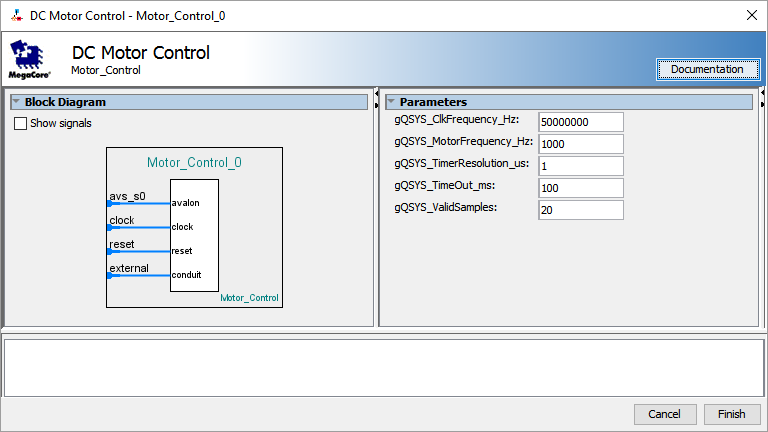
\includegraphics[width=1.00\textwidth]{./Parameter.png}
	\caption{IP Interface parameters}
	\label{fig:QSYS_IF_Parameters}
\end{figure}
\begin{center}
  \begin{tabular}{ | l | l | p{5cm} |}
	  \hline
		\textbf{Parameter} & \textbf{Target} & \textbf{Description} \\
    \hline
		gQSYS\_ClkFreqeuncy\_Hz & IP core & system clock frequency in hertz \\
		\hline
		gQSYS\_MotorFrequency\_Hz & MotorControl & motor switching frequency in hertz \\
		\hline
		gQSYS\_TimerResolution\_us & WheelEncoder & LSB of speed sensor impulse period value \\
		\hline
		gQSYS\_TimeOut\_us & WheelEncoder & within this time window the signal state must be stable \\
		\hline		
		gQSYS\_ValidSamples & WheelEncoder & valid Samples from speed sensor to guarantee stable edge detection\\
		\hline
  \end{tabular}
\end{center}
For details see functional description below.
\subsection{Register Mapping}
The data width of all used registers are 32bit
\begin{center}
  \begin{tabular}{ | l | c | c | l|}
    \hline
		\textbf{Address} & \textbf{Register} & \textbf{R/W} & \textbf{Description} \\
		\hline
		+0 & Control & R/W & Bit 0: Enable PWM \\
		 & & & Bit 1: Run otherwise Brake \\
		 & & & Bit 2: Reset new round detected signal\\
		\hline
		+1 & Status & R & Bit 0: new round detected (Reset see Control, Bit 2) \\
		& & & Bit 1: new round detected toggle \\
		\hline
		+2 & PWM & R/W & 10Bit Resolution Duty Cycle  \\
		\hline
		+3 & Speed & R & Impulse periode of speed sensor in us \\
		\hline
		+4 & Distance & R/W & Impulse counter, Write to address to set value \\
    \hline
		+5 & Error & R & Error counter of speed sensor unit \\
    \hline

  \end{tabular}
\end{center}

\section{Wheel Sensor module}
\subsection{WheelSensor}
Window method has been cancelled due to bad resolution and emc.

\subsection{WheelSensorTimer}

Frequency measurement: measures the elapsed time between two identical edges of sensor signal. Measured time in us is populated to register. Time out is defined to have finite sampling time period. Signal parameters are shown in figure \ref{fig:WheelEncoderTimer_Signal_Parameters}.

\begin{figure}[h]
	\centering
		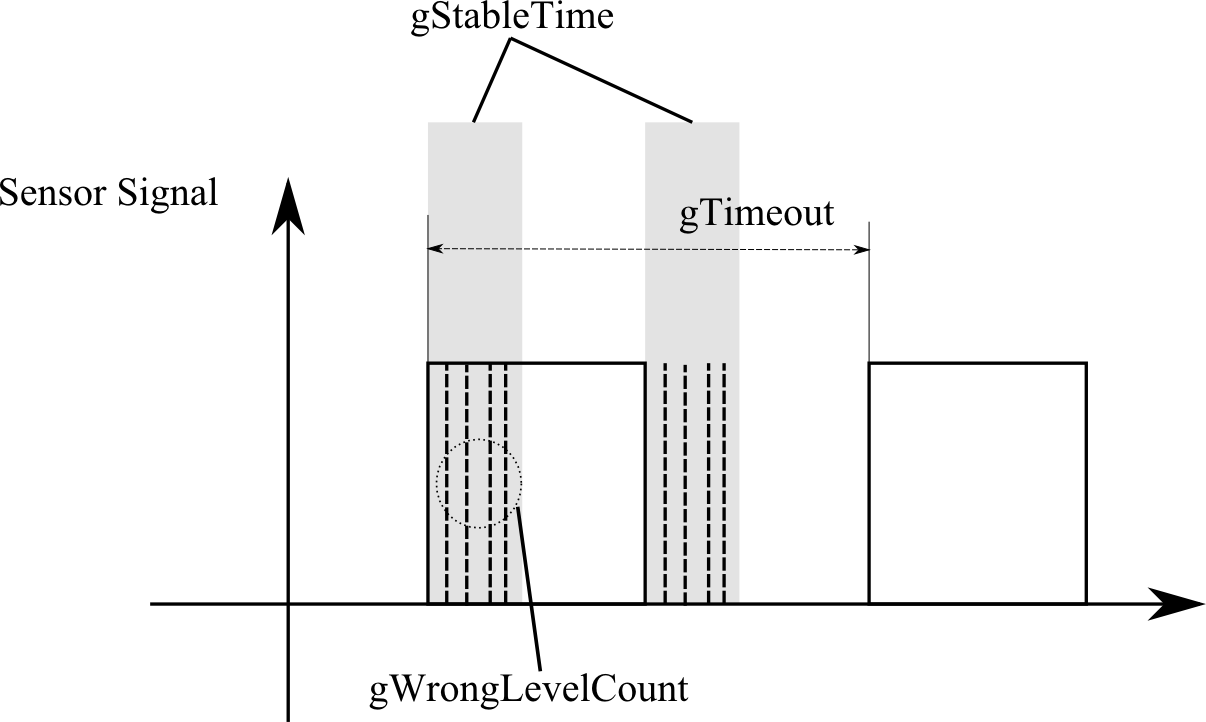
\includegraphics[width=1.00\textwidth]{./WheelEncoderTimer_Signal_Parameters.png}
	\caption{Signal parameters}
	\label{fig:WheelEncoderTimer_Signal_Parameters}
\end{figure}

\begin{figure}[h]
	\centering
		\includegraphics[angle = 90, height=1.00\textheight]{WheelEncoderWaveform.png}
	\caption{wheel encoder unit waveform from simulation}
	\label{fig:WheelEncoderWaveform}
\end{figure}

\subsubsection{Speed}
\emph{HINT:} If Register holds 0x0000 it will indicate zero speed.
$$ v = \frac{1}{Register[3]} \cdot  \frac{d \cdot \pi \cdot 10^{6}}{i}  = [\frac{m}{s}] $$
$ d=0,028 m,$
$ i=16 $

\subsubsection{Distance}
$$ x = {Register[4]} \cdot  \frac{d \cdot \pi}{i}  = [\frac{m}{s}] $$
$ d=0,028 m,$
$ i=16 $


\section{Round Sensor}
Sampling time 10us (default). Valid Samples 10.
2 Kind of signals: Reset by user and toggled see \ref{fig:ModRoundSensorWaveform}.
After detection of falling edge and rising edge at round sensor signal bit 0 and bit 1 in status register (+1) will be modified. Bit 0 will be set by sensor signal and reset by setting Bit 2 in control register (+0).

\begin{figure}[h]
	\centering
		\includegraphics[width=1.00\textwidth]{ModRoundSensorWaveform.png}
		\caption{Round Sensor waveform from simulation}
	\label{fig:ModRoundSensorWaveform}
\end{figure}


\section{Motor Control (PWM)}
10-Bit PWM Control

\begin{figure}[h]
	\centering
		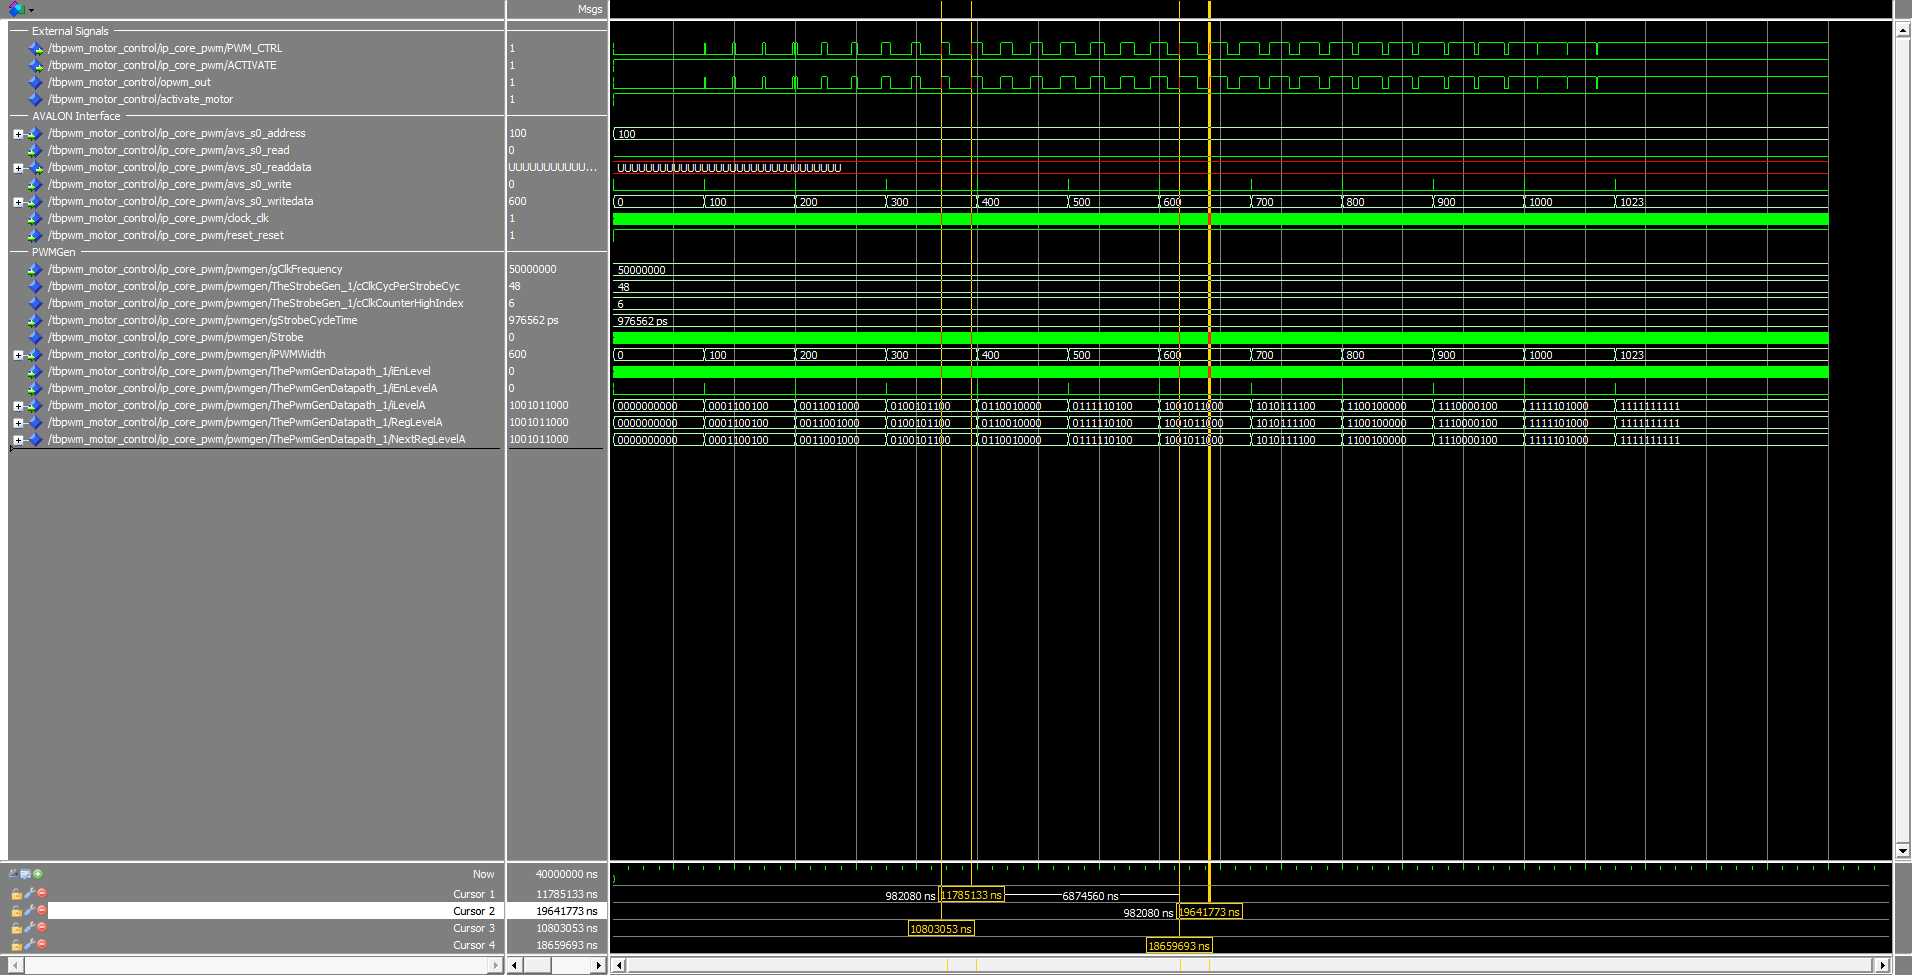
\includegraphics[angle = 90, height=1.00\textheight]{MotorControlWaveform.png}
	\caption{PWM Generation unit waveform from simulation}
	\label{fig:MotorControlWaveform}
\end{figure}


%%%%%%%%%%%%%%%%%%%%%%%%%%%%%%%%%%%%%%%%%%%%%%%%%%
\end {document}

